%%%%%%%%%%%%%%%%%%%%%%%%%%%%%%%%%%%%%%%%%
% Beamer Presentation
% LaTeX Template
% Version 1.0 (10/11/12)
%
% This template has been downloaded from:
% http://www.LaTeXTemplates.com
%
% License:
% CC BY-NC-SA 3.0 (http://creativecommons.org/licenses/by-nc-sa/3.0/)
%
%%%%%%%%%%%%%%%%%%%%%%%%%%%%%%%%%%%%%%%%%

%----------------------------------------------------------------------------------------
%   PACKAGES AND THEMES
%----------------------------------------------------------------------------------------

%\documentclass{beamer}
\documentclass[aspectratio=169]{beamer}
\mode<presentation> {

  % The Beamer class comes with a number of default slide themes
  % which change the colors and layouts of slides. Below this is a list
  % of all the themes, uncomment each in turn to see what they look like.

  %\usetheme{default}
  %\usetheme{AnnArbor}
  %\usetheme{Antibes}
  %\usetheme{Bergen}
  %\usetheme{Berkeley}
  %\usetheme{Berlin}
  %\usetheme{Boadilla}
  %\usetheme{CambridgeUS}
  %\usetheme{Copenhagen}
  %\usetheme{Darmstadt}
  %\usetheme{Dresden}
  %\usetheme{Frankfurt}
  %\usetheme{Goettingen}
  %\usetheme{Hannover}
  %\usetheme{Ilmenau}
  %\usetheme{JuanLesPins}
  %\usetheme{Luebeck}
  \usetheme{Madrid}
  %\usetheme{Malmoe}
  %\usetheme{Marburg}
  %\usetheme{Montpellier}
  %\usetheme{PaloAlto}
  %\usetheme{Pittsburgh}
  %\usetheme{Rochester}
  %\usetheme{Singapore}
  %\usetheme{Szeged}
  %\usetheme{Warsaw}

  % As well as themes, the Beamer class has a number of color themes
  % for any slide theme. Uncomment each of these in turn to see how it
  % changes the colors of your current slide theme.

  %\usecolortheme{albatross}
  %\usecolortheme{beaver}
  %\usecolortheme{beetle}
  %\usecolortheme{crane}
  %\usecolortheme{dolphin}
  %\usecolortheme{dove}
  %\usecolortheme{fly}
  %\usecolortheme{lily}
  %\usecolortheme{orchid}
  %\usecolortheme{rose}
  %\usecolortheme{seagull}
  %\usecolortheme{seahorse}
  \usecolortheme{whale}
  %\usecolortheme{wolverine}

  %\setbeamertemplate{footline} % To remove the footer line in all slides uncomment this line
  %\setbeamertemplate{footline}[page number] % To replace the footer line in all slides with a simple slide count uncomment this line

  %\setbeamertemplate{navigation symbols}{} % To remove the navigation symbols from the bottom of all slides uncomment this line
}
\usefonttheme[onlymath]{serif}
%\usepackage{epsfig}
\usepackage{graphicx} % Allows including images
\usepackage{booktabs} % Allows the use of \toprule, \midrule and \bottomrule in tables
\usepackage{multimedia} % 
%\usepackage{animate}
%\usepackage{tikz}
%\usepackage{lipsum}

\usepackage{tikz} 
\usetikzlibrary{tikzmark,overlay-beamer-styles,positioning,calc}
%\usetikzlibrary{tikzmark,
%\usetikzlibrary{tikzmark}
%\usetikzlibrary{arrows,shapes}
%\newcommand{\tikzmark}[1]{\tikz[remember picture] \node[coordinate] (#1) {#1};}
\newcommand{\be}{\begin{equation*}}
\newcommand{\ee}{\end{equation*}}
\newcommand{\ol}{\overline}
\newcommand{\p}{\partial}
\newcommand{\pdv}[2]{\frac{\partial \, #1}{\partial #2}}
\newcommand{\etal}{ {\it et al.} }
%----------------------------------------------------------------------------------------
%   TITLE PAGE
%----------------------------------------------------------------------------------------

\title[CHARTS]{Candidate CHARTS Model Summary} % The short title appears at the bottom of every slide, the full title is only on the title page

\author[]{Brad Johnson\\Liz Holzenthal\\Rusty Permenter \\Kevin Hodgens } % Your name
\institute[ERDC] % Your institution as it will appear on the bottom of every slide, may be shorthand to save space
{USACE Engineering Research and Devlelopment Center \\ % Your institution for the title page
\medskip
\textit{} % Your email address
}
%\date{\today} % Date, can be changed to a custom date
\date{\vspace*{-0cm}\\ Oct, 2024} % Date, can be changed to a custom date

\begin{document}

\begin{frame}
  %\titlepage % Print the title page as the first slide
  \begin{columns}[c] % The "c" option specifies centered vertical alignment while the "t" option is used for top vertical alignment
    
    \column{.3\textwidth} % Left column and width
    \titlepage % Print the title page as the first slide
%%     \vspace*{-1cm}
%%     \begin{center}
%% District PDT:\\
%% Kelly Legault (SAJ)\\
%% Gabriel Todaro (SAJ)
%%     \end{center}
    \column{.7\textwidth} % Right column and width
    \begin{figure}
            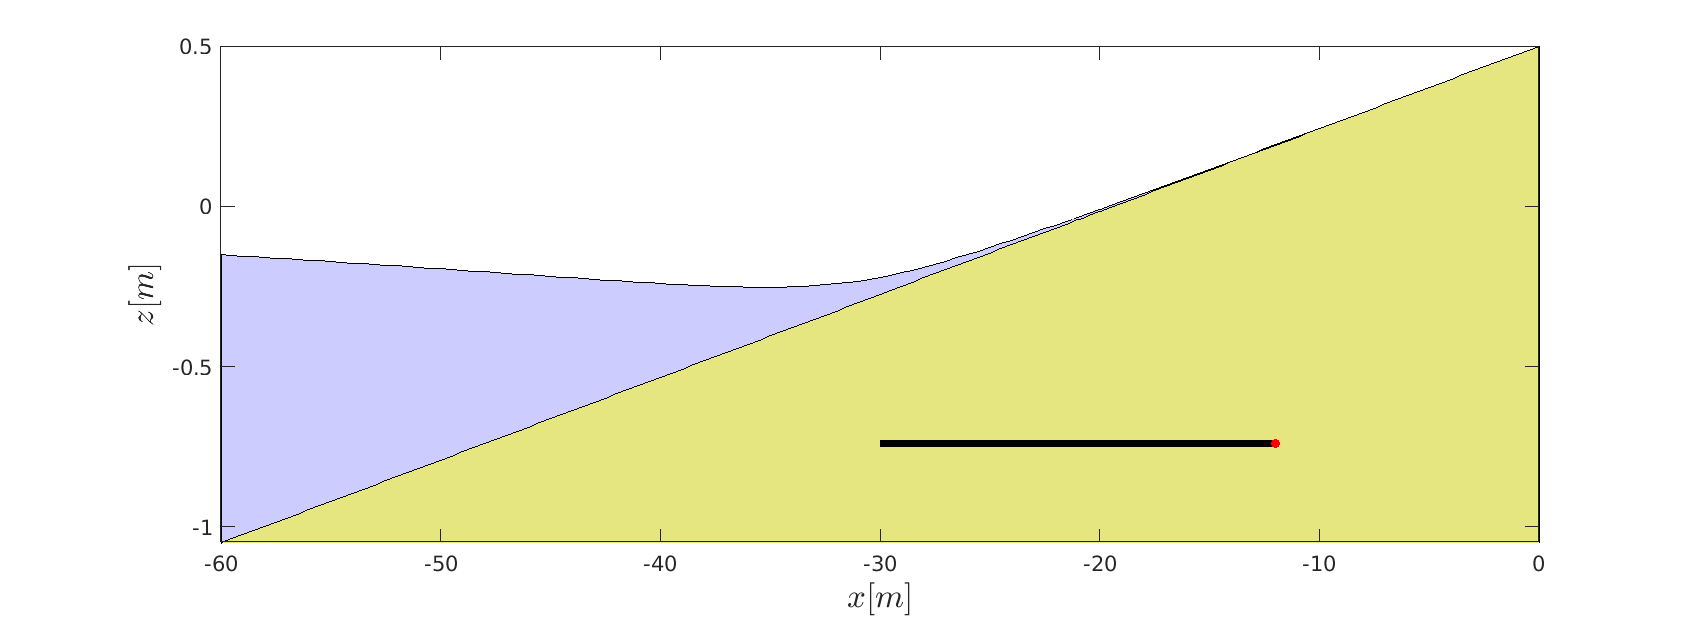
\includegraphics[width=1\linewidth]{./present.png}
      %\includegraphics[trim={0 1cm 0 0},clip,width=0.9\linewidth]{./breaking-wave-on-the-beach.jpg}
    \end{figure}
    
  \end{columns}
\end{frame}
%%%%%%%%%%%%%%%%%%%%%%%%%%%%%%%%%%%%%%%%%%%%%%%%%%%%%%%%%%%%%%%%%%%%%%%%%%%%%%%%%%%%%%%%%%%%%%%%%%%%

\begin{frame}
  \frametitle{Model Objectives}

  The CHART effort requires  simple, stable, and computationally efficient hydrodynamics framework that can be customized to meet USACE needs.
 \begin{columns}[c] % 
    
   \column{.5\textwidth} % Left column and width

  First incarnation model:
 \begin{itemize}
 \item One-dimensional
 \item Phase-averaged but low-frequency resolving
 \item Based on NLSW 
 \item Heuristic wet/dry
 \item Emphasis on simple and efficient
 \item Somewhat numerically diffusive, but requires additional 'viscosity' if we extend to short waves--see angry wave fronts for 10 sec waves
   \end{itemize}
   \column{.5\textwidth} % Left column and width
    \begin{figure}
      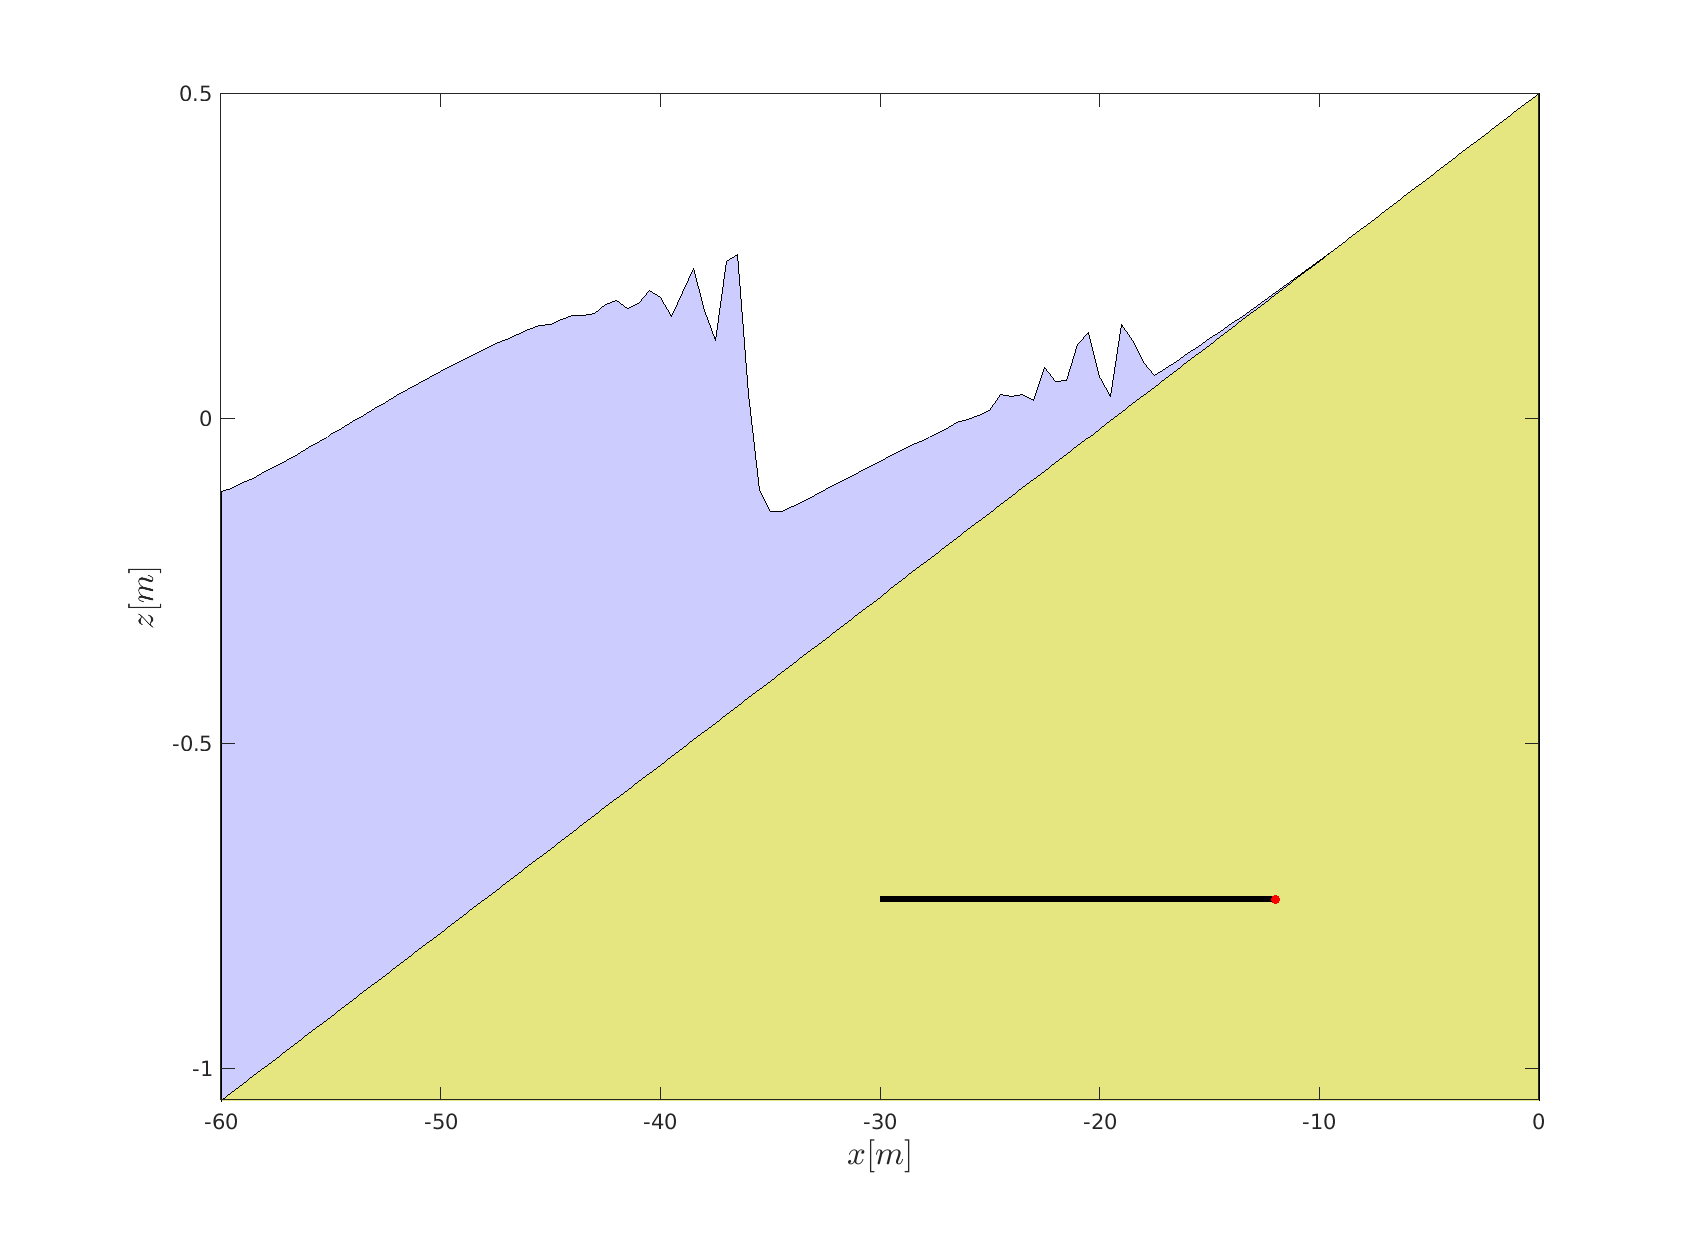
\includegraphics[width=1\linewidth]{./shortwave.png}
    \end{figure}

 \end{columns}
 \end{frame}
%%%%%%%%%%%%%%%%%%%%%%%%%%%%%%%%%%%%%%%%%%%%%%%%%%%%%%%%%%%%%%%%%%%%%%%%%%%%%%%%%%%%%%%%%%%%%%%%%%%%
\begin{frame}
  \frametitle{Model Formulation}
\begin{align*}
\pdv{h}{t} + \pdv{q}{x} -\textcolor{blue}{\frac{k}{\mu}\pdv{\hat{P}}{z}} &= 0\\
\pdv{q}{t} + \pdv{}{x}\left\{ \frac{q^2}{h} + \textcolor{blue}{\frac{S_{xx}}{\rho}} \right\} &= - g h \pdv{\eta}{x} -\frac{\tau_{b}}{\rho}  +\frac{\tau_{s}}{\rho}  
\end{align*}

Represents
\begin{itemize}
 \item A NLSW set ( hydrostatic, depth-uniform, etc)
 \item \textcolor{blue}{Infiltration} by Darcy's law
 \item \textcolor{blue}{Steady Waves} through rad stress, no IG generation, no W/C interaction
 \item Quadratic wind stress
    \item Quadratic current-dominated bottom shear stress
\end{itemize}

\end{frame}
%%%%%%%%%%%%%%%%%%%%%%%%%%%%%%%%%%%%%%%%%%%%%%%%%%%%%%%%%%%%%%%%%%%%%%%%%%%%%%%%%%%%%%%%%%%%%%%%%%%%
\begin{frame}
  \frametitle{Numerical Apparatus }

  FD Soln:
\begin{itemize}
 \item Time: 1st order by Fisher's method
 \item Pressure: 2nd order centered, except at boundaries
 \item Advective: 1st order upwinding 
\end{itemize}


\begin{columns}[c] % The "c" option specifies centered vertical alignment while the "t" option is used for top vertical alignment
    
  \column{.5\textwidth} % Left column and width
  Left boundary options
  \begin{itemize}
  \item Generation
  \item Transmitting
  \item Gen/Trans
  \item Reflective
  \item User-defined water level
  \end{itemize}

  \column{.5\textwidth} % Left column and width
  Right boundary options
  \begin{itemize}
  \item Reflective
  \item \textcolor{blue}{Tail-water}
  \end{itemize}
\end{columns}
\end{frame}
%%%%%%%%%%%%%%%%%%%%%%%%%%%%%%%%%%%%%%%%%%%%%%%%%%%%%%%%%%%%%%%%%%%%%%%%%%%%%%%%%%%%%%%%%%%%%%%%%%%%
\begin{frame}
  \frametitle{Runup on Planar Slope}
  With periodic offshore BC of 150s, gen/trans
  \centering
    \movie[externalviewer]{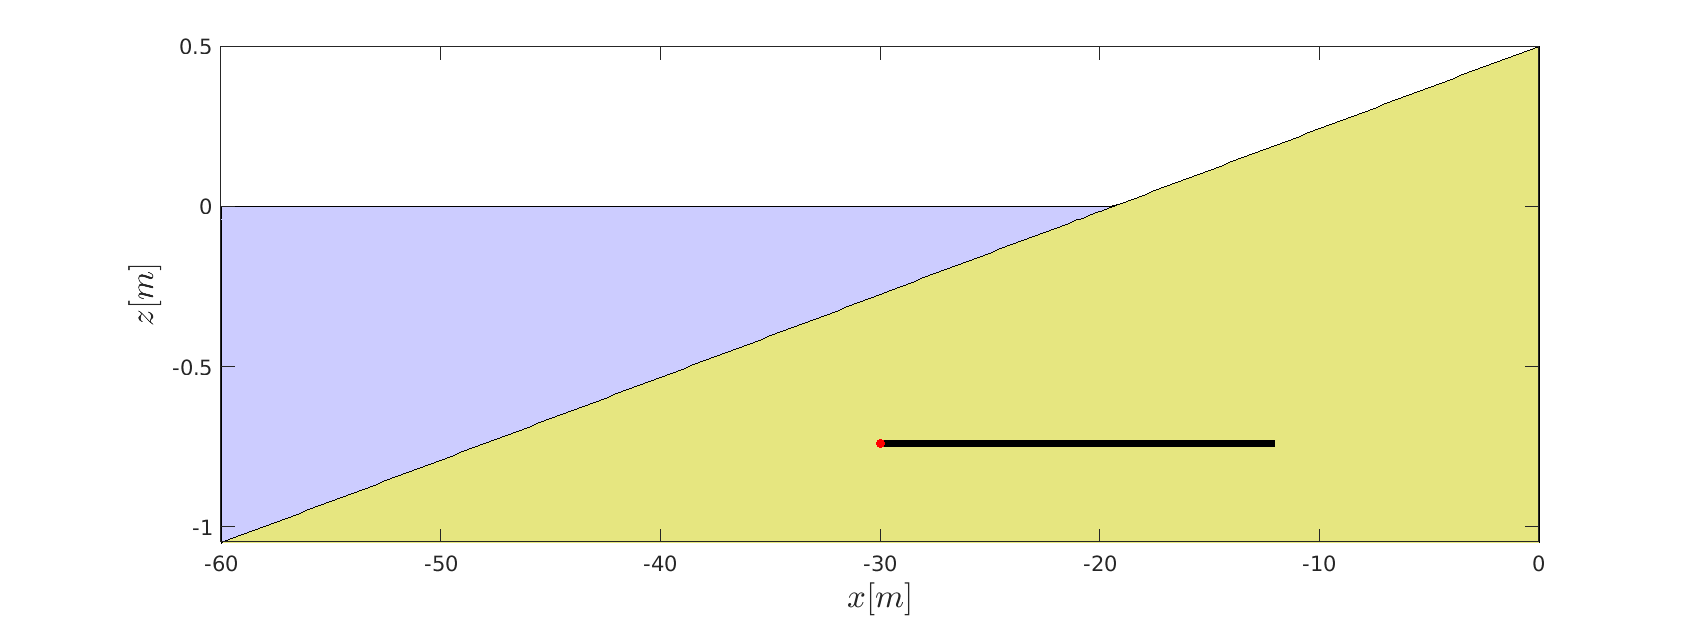
\includegraphics[width=\textwidth, keepaspectratio]{planar.png}}{planar.avi}
\end{frame}
%%%%%%%%%%%%%%%%%%%%%%%%%%%%%%%%%%%%%%%%%%%%%%%%%%%%%%%%%%%%%%%%%%%%%%%%%%%%%%%%%%%%%%%%%%%%%%%%%%%%
\begin{frame}
  \frametitle{Left and Right MBC}
  Fully reflective BC on Left and Right + initial displacement of $\eta$
    \centering
    \movie[externalviewer]{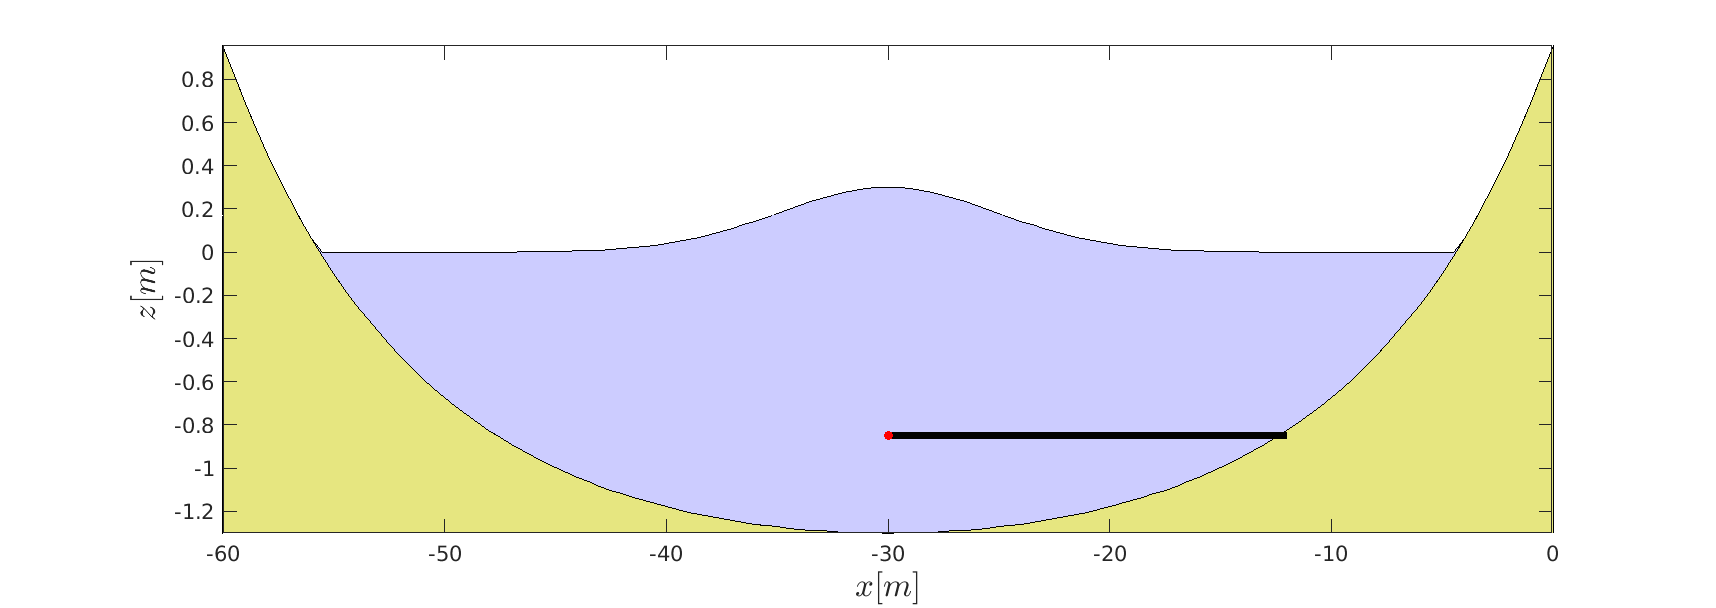
\includegraphics[width=\textwidth, keepaspectratio]{leftandrightmbc.png}}{leftandrightmbc.avi}
\end{frame}
%%%%%%%%%%%%%%%%%%%%%%%%%%%%%%%%%%%%%%%%%%%%%%%%%%%%%%%%%%%%%%%%%%%%%%%%%%%%%%%%%%%%%%%%%%%%%%%%%%%%
\begin{frame}
  \frametitle{Wind-driven Setup}
  Unrealistically large $\tau_s$
    \centering
    \movie[externalviewer]{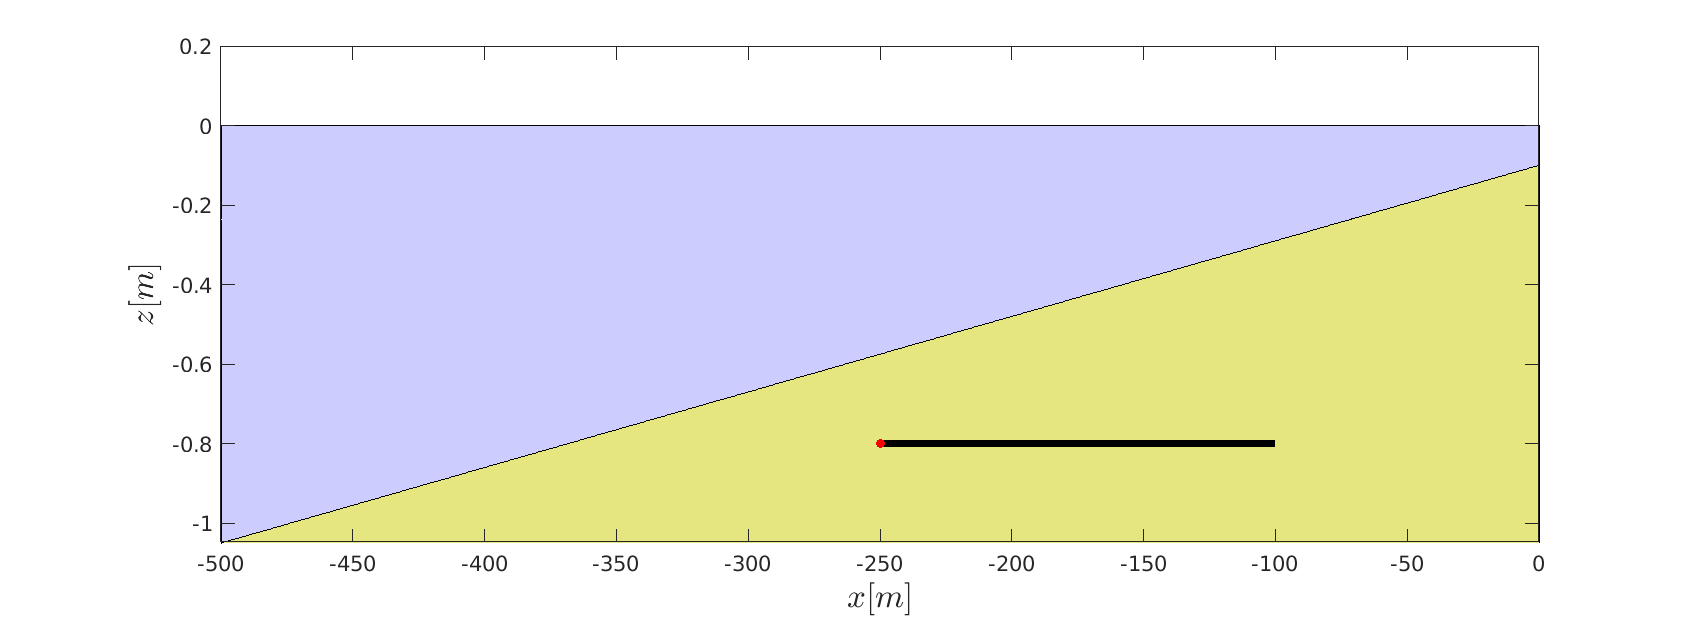
\includegraphics[width=\textwidth, keepaspectratio]{wind.png}}{wind.avi}
\end{frame}
%%%%%%%%%%%%%%%%%%%%%%%%%%%%%%%%%%%%%%%%%%%%%%%%%%%%%%%%%%%%%%%%%%%%%%%%%%%%%%%%%%%%%%%%%%%%%%%%%%%%
\begin{frame}
  \frametitle{Ponding}
  Overtopping capture, but no infiltration
    \centering
    \movie[externalviewer]{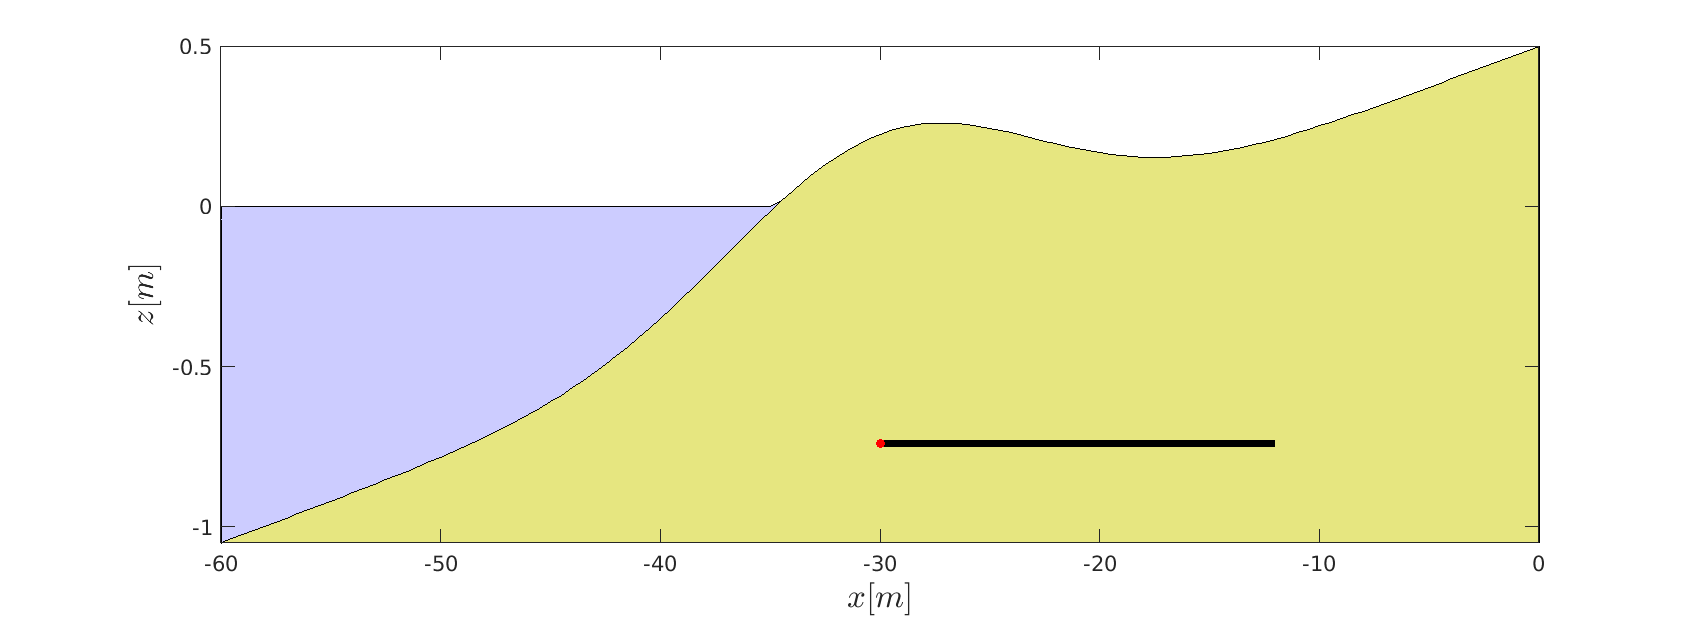
\includegraphics[width=\textwidth, keepaspectratio]{ponding.png}}{ponding.avi}
\end{frame}
%%%%%%%%%%%%%%%%%%%%%%%%%%%%%%%%%%%%%%%%%%%%%%%%%%%%%%%%%%%%%%%%%%%%%%%%%%%%%%%%%%%%%%%%%%%%%%%%%%%%
\begin{frame}
  \frametitle{Wave forcing}
  A one-line wave model:
  \begin{equation*}
    H_{i+1}=\min{\left(\left\{ H_i^2 \frac{c_i n_i}{c_{i+1} n_{i+1}}\right\}^{1/2},\gamma h_i\right)}
  \end{equation*}
  
    \centering
    \movie[externalviewer]{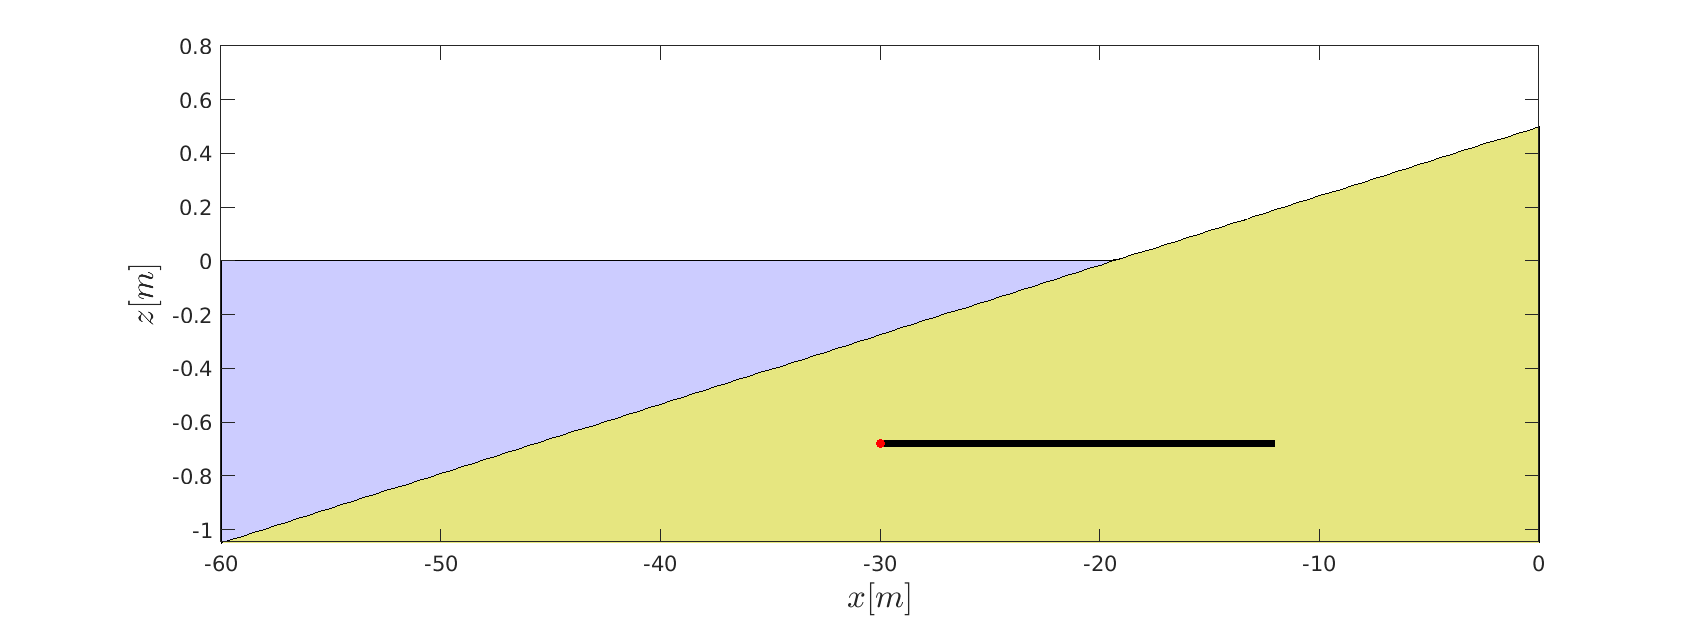
\includegraphics[width=\textwidth, keepaspectratio]{planarwithwaves.png}}{planarwithwaves.avi}
\end{frame}
%%%%%%%%%%%%%%%%%%%%%%%%%%%%%%%%%%%%%%%%%%%%%%%%%%%%%%%%%%%%%%%%%%%%%%%%%%%%%%%%%%%%%%%%%%%%%%%%%%%%



\begin{frame}
  \frametitle{Next Steps}
  \begin{columns}[c] % The "c" option specifies centered vertical alignment while the "t" option is used for top vertical alignment
    
    \column{.5\textwidth} % Left column and width

    \underline{Major concerns}
    
    \begin{itemize}
    \item No morphology
    \item Overtopping doesn't include impact of waves (other than forced MWL)
    \item No 2DH
    \item Runtimes: 1 day simulation $\sim$ 1 min 
    \item No account for reflective structures
    \item Not perfectly conservative
    \end{itemize}
    \column{.5\textwidth} % Left column and width
    
    \underline{Minor concerns}
    
    \begin{itemize}
    \item No infiltration
    \item Constant waves at boundary
    \item no impact on waves on $\tau_b$
    \end{itemize}
  \end{columns}
  
  \center{\Large{Kill or Continue?}}
  
\end{frame}
%%%%%%%%%%%%%%%%%%%%%%%%%%%%%%%%%%%%%%%%%%%%%%%%%%%%%%%%%%%%%%%%%%%%%%%%%%%%%%%%%%%%%%%%%%%%%%%%%%%%
\end{document}
